\section{Introduction}
\label{sec:intro}

Multimodal large language models (MLLMs) are increasingly deployed as agents that complete multi-step tasks by perceiving and acting on graphical user interfaces (GUIs)~\citep{cheng2024seeclick,guiowl2025}.
%
At each step, a GUI agent processes the high-resolution screenshot together with context accumulated from earlier interactions~\citep{tian2025mmina}.
%
As the trajectory unfolds, visual computation grows to dominate the inference cost.
%
Each historical screenshot carries a large number of visual tokens and recurs across successive steps, inflating both computation and memory~\citep{xie2024osworld}.
%
As shown in Fig.~\ref{fig:evidence} (a), cache reuse mitigates the temporal redundancy across frames by limiting past computation~\citep{zheng2024sglang}.
%
However, this mechanism operates at frame granularity and leaves substantial spatial redundancy within each retained screenshot.
%
The core problem therefore becomes deciding which visual tokens enter the reusable state of each frame.
\begin{figure}[t]
    \centering
    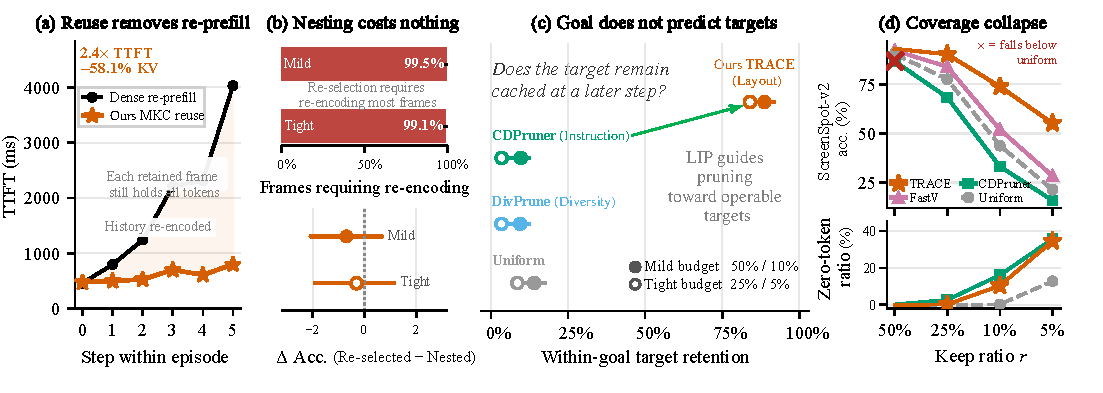
\includegraphics[width=0.99\linewidth]{figures/fig2_evidence.pdf}
    \vspace{-0mm}
    \caption{%
    \textbf{Motivation of our proposed TRACE.} %
    \textbf{(a)}~Reusing the cache removes repeated prefill and lowers latency. %
    \textbf{(b)}~Independent re-selection demands re-encoding on most frames, while the nested order costs no accuracy. %
    \textbf{(c)}~Instruction-based pruning misses the target in later steps while layout-based pruning retains it. %
    \textbf{(d)}~Concentrating the budget on salient regions loses spatial coverage.}
    \label{fig:evidence}
\end{figure}

Training-free visual token pruning has emerged as an effective way to reduce this redundancy.
%
For example, FastV~\citep{chen2024fastv} prunes tokens by attention distribution.
%
DivPrune~\citep{alvar2025divprune} and CDPruner~\citep{zhang2025cdpruner} select for feature diversity or instruction relevance.
%
Besides, PruMerge~\citep{shang2025prumerge} merges redundancy into synthetic summaries.
%
These approaches are effective because the selection can be recomputed whenever the query changes.
%
Multi-step GUI serving breaks this premise once visual state becomes reusable, because each screenshot is encoded and written into the session cache only at its first prefill.
%
Later steps read history from that cache rather than pixels, so tokens dropped at the single write are absent for every future query and can only be recovered by re-encoding the frame.
%
\textbf{Visual token pruning thus shifts from revisable selection to irreversible write-time commitment of visual evidence.}
%
Under this commitment, each frame should be admitted once before prefill, reused while current, and contracted when it becomes history.
%
Contraction can only drop tokens from the committed state, so the historical keep sets should nest inside the current one.
%
Pruning therefore must output a nested order whose prefixes realize every budget.
%
As shown in Fig.~\ref{fig:evidence} (b), re-selection demands re-encoding on most frames, whereas enforcing the nested order costs no accuracy.
%
We term this regime \emph{lifecycle-aware visual pruning} and formulate its decision as \emph{write-time visual evidence commitment under trajectory uncertainty}.

This formulation exposes two distinct challenges.
%
The first is trajectory uncertainty.
%
The task goal is known at admission, yet the fine-grained targets along the trajectory remain unknown.
%
Write-time admission must therefore commit evidence before those later targets appear.
%
Among the signals available at that moment, feature diversity is query-independent yet does not separate operable regions from background.
%
By contrast, the interface layout offers operable regions before any demand is observed.
%
As shown in Fig.~\ref{fig:evidence} (c), when a screen recurs under the same goal, instruction-selected tokens miss the later target, whereas layout-selected tokens still cover it.
%
Beyond present-step cues, trajectory-robust admission should therefore also incorporate this layout prior.
%
Independently, the second challenge is spatial coverage under tight budgets.
%
Biased token pruning concentrates on a few salient regions, leaving other operable regions with zero support and thus unavailable to the agent.
%
As shown in Fig.~\ref{fig:evidence} (d), such biased keeps leave a growing uncovered area and eventually fall below uniform sampling as the budget tightens~\citep{deng2025scope,xu2026score}.
%
Beyond importance concentration, tight-budget admission must therefore also preserve spatial coverage.

Motivated by these observations, we propose \textbf{\method{}}, a \emph{\textbf{T}rajectory-\textbf{r}obust \textbf{A}dmission and \textbf{C}overage-aware \textbf{E}vidence ordering} framework for efficient GUI agents.
%
Specifically, \method{} comprises four key components: \textbf{Layout-derived Interaction Prior (\lmp{})}, \textbf{Nested Evidence Ordering (\nwe{})}, \textbf{Native-token Coverage Repair (\awc{})}, and \textbf{Monotone KV Contraction (\kvr{})}.
%
First, \lmp{} maps layout detections into an interaction prior, enabling admission to favor operable regions before later targets appear.
%
Second, \nwe{} fuses this prior with instruction relevance and feature novelty into one nested order, so every tighter budget is realized as a prefix rather than by re-selection.
%
Third, \awc{} restores spatial coverage with native tokens while preserving that nested order.
%
Finally, \kvr{} contracts each retiring frame to its history prefix and replays the retained native rows in the next prefill.
%
Together, these components commit visual evidence once at admission and contract it monotonically thereafter.
%
In this way, \method{} realizes lifecycle-aware visual pruning under trajectory uncertainty for efficient GUI agents.
%
Extensive experiments across six GUI benchmarks covering single-step and multi-step settings, including multiple model scales and a cross-family backbone, verify the effectiveness of \method{}.
%
Overall, our contributions can be summarized as follows.
\begin{itemize}
\item We formulate \emph{lifecycle-aware visual pruning} as \emph{write-time visual evidence commitment under trajectory uncertainty}. Once visual state is reusable, pruning becomes an irreversible admission with nested keep sets across budgets, exposing two challenges of committing evidence before later targets appear and preserving spatial coverage under tight budgets.
\item We propose \method{}, a training-free framework that commits visual evidence once and contracts it monotonically thereafter. \lmp{} injects a query-independent layout prior, \nwe{} builds one nested evidence order, \awc{} restores native-token spatial coverage, and \kvr{} turns the admitted order into reusable session state without re-encoding historical frames.
\item Extensive experiments across six GUI benchmarks verify the effectiveness of \method{} under single-step and multi-step settings, multiple model scales, and a cross-family backbone.
\end{itemize}
